% =====================================================================
% EEEM068 Applied Machine Learning - Human Sentiment Analysis (MSCTD En-De)
% IEEE Conference style, double column, 5 pages excluding references.
% =====================================================================
\documentclass[conference]{IEEEtran}
\IEEEoverridecommandlockouts

% --- Packages ---------------------------------------------------------
\usepackage{cite}
\usepackage{amsmath,amssymb,amsfonts}
\usepackage{algorithmic}
\usepackage{graphicx}
\usepackage{textcomp}
\usepackage{xcolor}
\usepackage{booktabs}
\usepackage{multirow}
\usepackage{subcaption}
\usepackage{url}
\usepackage{hyperref}

\graphicspath{{figures/}}

% --- Title & Authors --------------------------------------------------
\title{Multimodal Human Sentiment Analysis on the MSCTD Dataset:\\
Combining Face-Level, Full-Image and Vision-Language Cues}

\author{
\IEEEauthorblockN{Shaik Sameer\IEEEauthorrefmark{1},
                  Ammineni Harshitha\IEEEauthorrefmark{1},
                  Tharigopula Sai Teja\IEEEauthorrefmark{1},
                  Kakumanu Ravi Teja\IEEEauthorrefmark{1},
                  Mosi Curran\IEEEauthorrefmark{1}}
\IEEEauthorblockA{\IEEEauthorrefmark{1}EEEM068 Applied Machine Learning, University of Surrey, UK}
}

\begin{document}
\maketitle

% --- Abstract (5\%) ---------------------------------------------------
\begin{abstract}
We address three-class sentiment classification (negative, neutral, positive)
on the English--German subset of the MSCTD dataset. We design a layered
pipeline that (i) extracts faces with MTCNN and trains a ResNet-18
face-level classifier, (ii) characterises robustness under frequency,
spatial and brightness degradations and re-trains with augmentation,
(iii) extracts full-image scene features with a frozen ResNet-50 and
trains a custom MLP head, and (iv) fuses face probabilities, full-image
probabilities and the number of detected faces through a small MLP. As
extra credit, we additionally fine-tune a CLIP image+text classifier
that consumes both modalities. Results indicate that (a) full-image
context helps in the dominant neutral class, (b) augmented training
substantially closes the gap on degraded inputs, and (c) the fusion
model outperforms either single-source model in macro-F1, particularly
when no face is detectable. The CLIP multimodal model is competitive
without retraining the encoders. Code and weekly contribution logs are
released in our private GitHub repository.
\end{abstract}

\begin{IEEEkeywords}
sentiment analysis, MSCTD, MTCNN, ResNet, CLIP, multimodal fusion,
robustness, transfer learning.
\end{IEEEkeywords}

% =====================================================================
% I. Introduction (10\%)
% =====================================================================
\section{Introduction}\label{sec:intro}
Human sentiment analysis from images is harder than from text because
visual sentiment cues are sparse, ambiguous and entangled with scene
context. The MSCTD dataset~\cite{msctd} is a multimodal chat-translation
corpus that pairs short utterances with the visual scene in which they
were uttered, providing fine-grained sentiment labels (negative, neutral,
positive). Working with the English--German (En-De) split, we tackle a
3-class classification task that brings together face analysis, transfer
learning, robustness and fusion -- all topics covered in EEEM068.

Our contributions are: (i) a clean MTCNN~\cite{mtcnn} extraction pipeline
with multiple-/no-face handling; (ii) a controlled robustness study
across the three degradation families requested by the brief; (iii) a
frozen-backbone full-image model that adds complementary scene context;
(iv) a late-fusion MLP that ingests face probabilities, image
probabilities and the number of detected faces; and (v) a CLIP-based
multimodal classifier that uses both image and text. The rest of the
paper is organised as follows: Section~\ref{sec:lit} reviews related
work, Section~\ref{sec:method} details our methodology,
Section~\ref{sec:exp} presents the experimental results, and
Section~\ref{sec:conc} concludes.

% =====================================================================
% II. Literature Review (15\%) - minimum 5 papers
% =====================================================================
\section{Literature Review}\label{sec:lit}
\textbf{Image classification backbones.} ResNet~\cite{he2016deep}
introduced residual connections that train substantially deeper CNNs;
ResNet-50 remains a strong default for transfer learning. Vision
Transformer~\cite{dosovitskiy2020vit} and Swin Transformer~\cite{liu2021swin}
later showed that pure attention-based models match or surpass CNNs
once enough pretraining data is available.
\textbf{Face detection and recognition.} MTCNN~\cite{mtcnn} casts face
detection and alignment as a cascade of three CNNs and is the de-facto
standard inside facenet-pytorch. FaceNet~\cite{schroff2015facenet}
provides discriminative face embeddings via triplet loss.
\textbf{Multimodal sentiment.}
Baltru{\v s}aitis et al.~\cite{baltrusaitis2018multimodal} survey
multimodal machine learning and identify alignment, fusion and
co-learning as the core challenges. CLIP~\cite{radford2021clip} aligns
image and text embeddings through 400M-pair contrastive pretraining and
has become a strong off-the-shelf multimodal feature extractor. LXMERT
\cite{tan2019lxmert} and ClipBERT~\cite{lei2021clipbert} explore
cross-attention transformers that jointly encode image regions and
text. \textbf{MSCTD.} Liang et al.~\cite{msctd} introduced the dataset
used here together with a multimodal sentiment-aware translation
baseline.

% =====================================================================
% III. Methodology (20\%)
% =====================================================================
\section{Methodology}\label{sec:method}

\subsection{Dataset and splits}
We use only the En-De portion of MSCTD. We pool the official
train/dev/test splits and re-stratify into a 70/15/15 split on the
sentiment label, fixing the random seed for reproducibility.
Fig.~\ref{fig:cls} reports the resulting class distribution.
\begin{figure}[t]
\centering
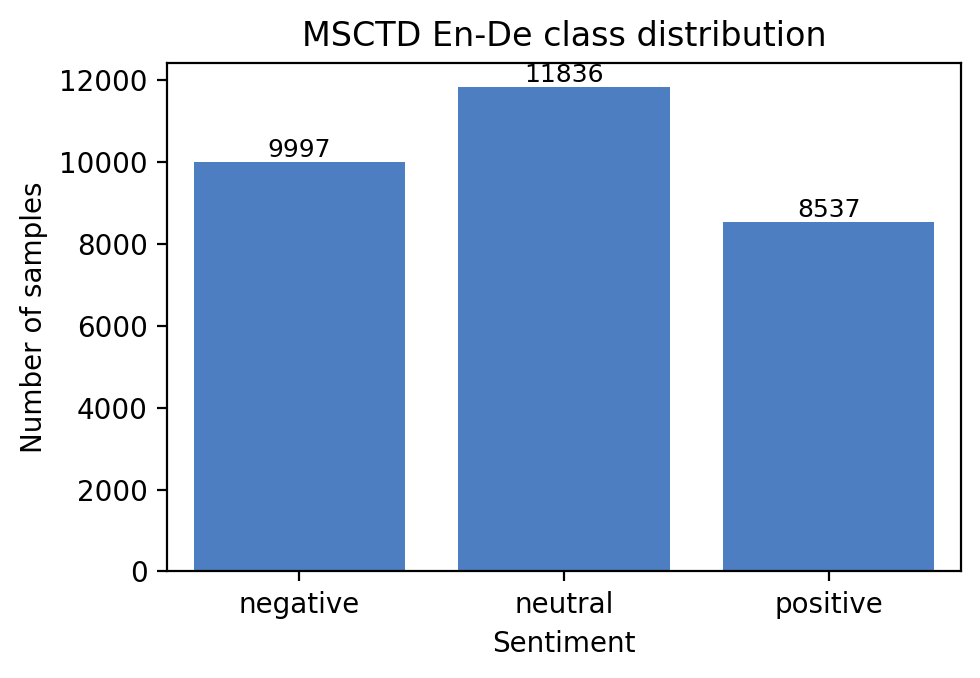
\includegraphics[width=0.95\linewidth]{class_distribution.png}
\caption{Class distribution of the MSCTD En-De subset.}\label{fig:cls}
\end{figure}

\subsection{Face-based model (Part 1)}
We use MTCNN~\cite{mtcnn} to detect every face in each image, crop with
margin and resize to $224{\times}224$. A ResNet-18 with ImageNet
weights is fine-tuned end-to-end with cross-entropy loss and inverse-frequency
class weights. Multi-face images contribute every face as an independent
training example; at inference time we average the per-face softmax
probabilities to obtain a single image-level prediction. Images with no
detected faces are flagged via \texttt{face\_detected\_flag}; for them
the fusion model uses the training-prior over labels in place of a face
probability.

\subsection{Robustness study (Part 2)}
We define three degradation families (Fig.~\ref{fig:aug}):
\emph{brightness} (multiplicative brightness/contrast jitter),
\emph{spatial} (rotation, affine translation, random crop, flip), and
\emph{frequency} (Gaussian blur, JPEG re-compression, Gaussian noise).
We run three controlled experiments: (A) train and test on original
faces; (B) train on original, test on degraded; (C) retrain with a
50\% probability of degrading each face per epoch and test on both
original and degraded sets.
\begin{figure}[t]
\centering
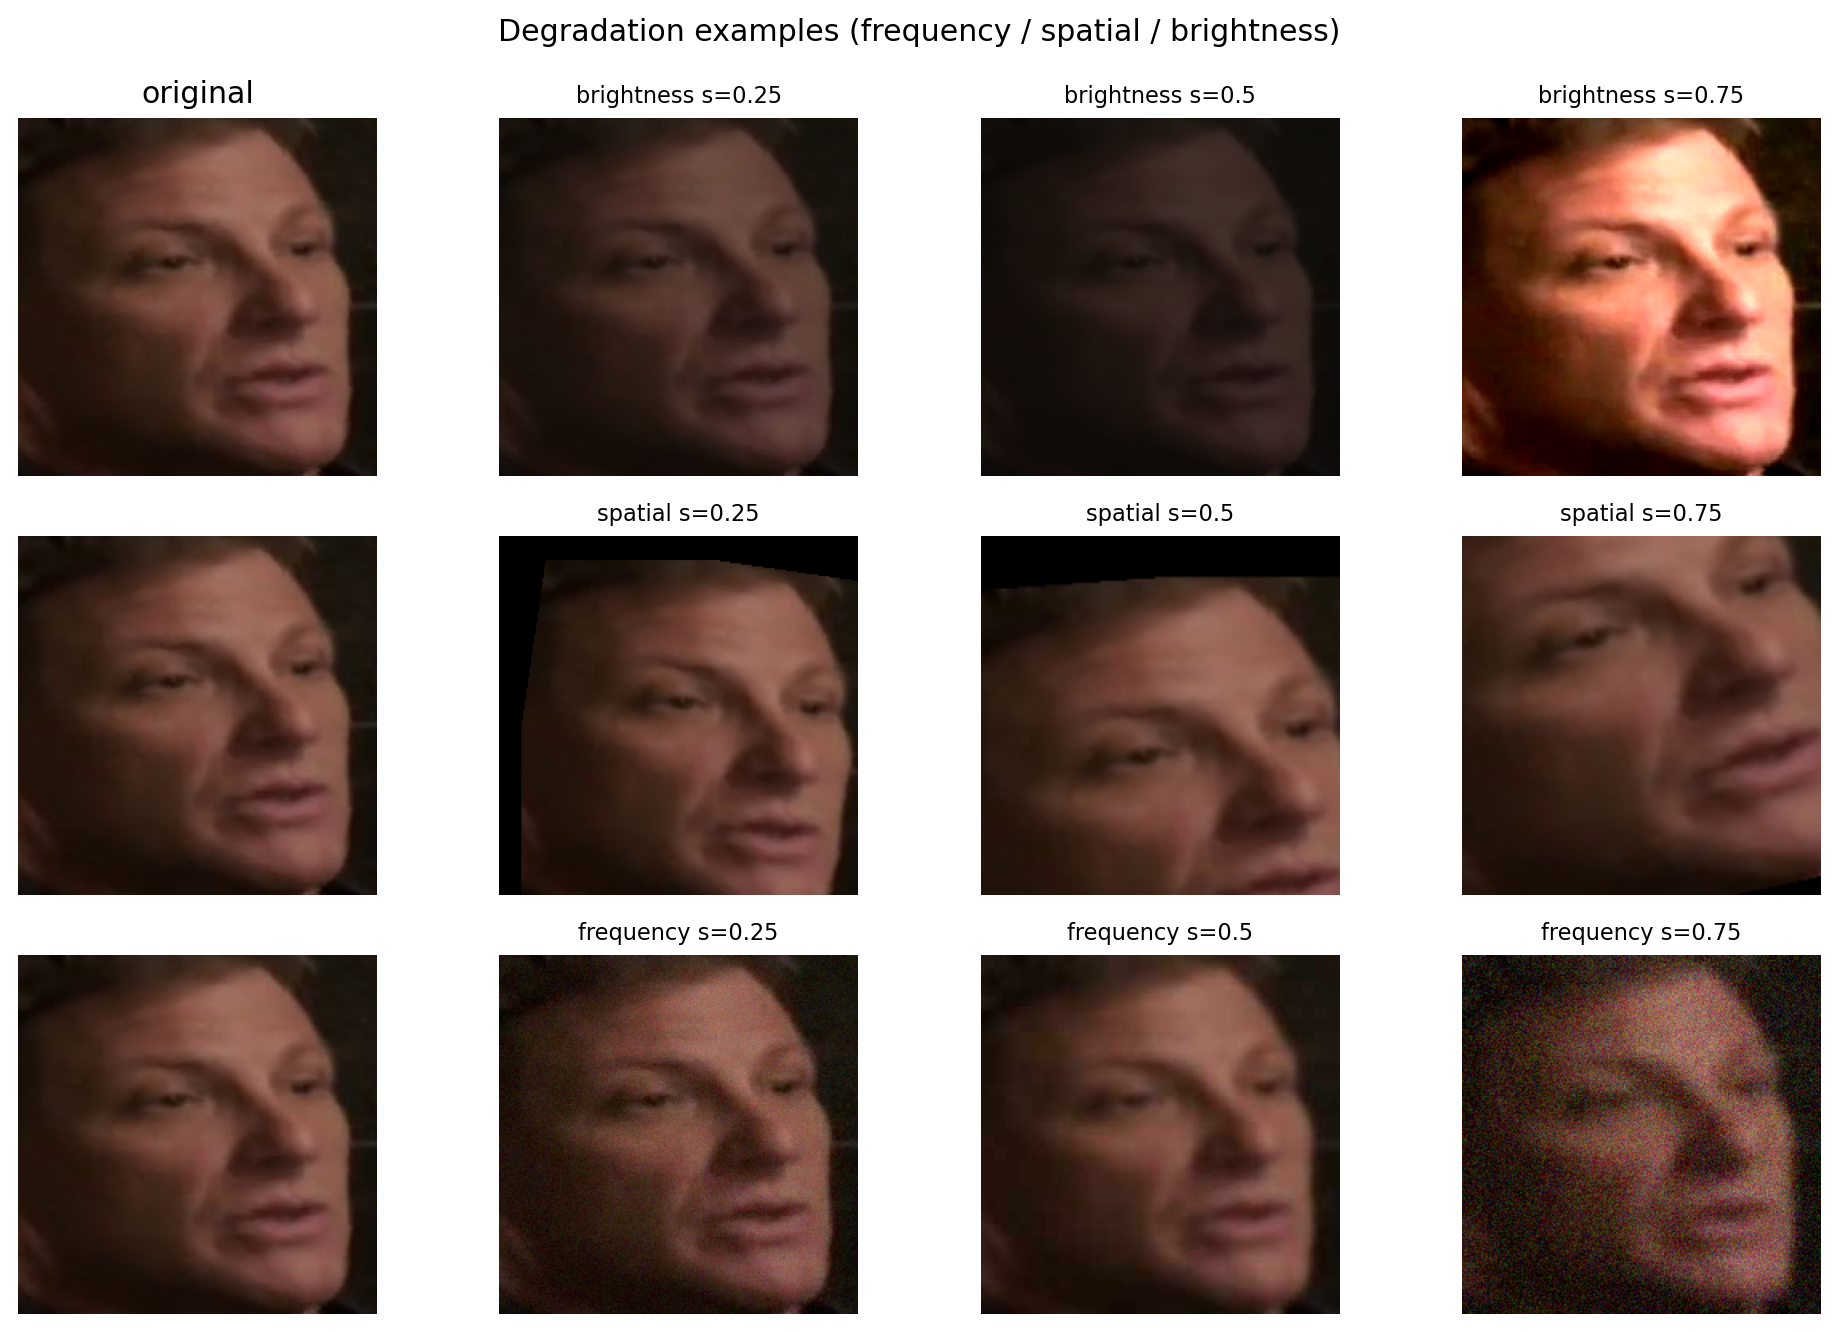
\includegraphics[width=0.98\linewidth]{augmentation_examples.png}
\caption{Three families of degradations applied to a sample face.}\label{fig:aug}
\end{figure}

\subsection{Full-image transfer learning (Part 3)}
A ResNet-50 backbone (ImageNet weights) is \emph{frozen} and used as a
feature extractor on the full $224{\times}224$ image. Its 2048-dim
output feeds an MLP \texttt{[Linear(2048,512)-ReLU-Drop(0.3)-Linear(512,128)-ReLU-Drop(0.2)-Linear(128,3)]}.
Only the MLP is trainable, satisfying the project constraint.

\subsection{Fusion model (Part 4)}
The fusion model is an 8$\to$32$\to$16$\to$3 MLP whose input is
$[\,p_{\text{face}}^{neg},p_{\text{face}}^{neu},p_{\text{face}}^{pos},
p_{\text{img}}^{neg},p_{\text{img}}^{neu},p_{\text{img}}^{pos},
\bar n,\,f\,]$, where $\bar n$ is the number of detected faces capped
at $5$ and rescaled to $[0,1]$, and $f\in\{0,1\}$ is the face-detected
flag. This late-fusion design lets the network learn how much to trust
each stream conditional on whether faces are visible.

\subsection{Extra credit: CLIP multimodal}
We use \texttt{openai/clip-vit-base-patch32}~\cite{radford2021clip} to
encode the image and the (English) utterance into 512-dim embeddings,
concatenate them, and train a small MLP head. The CLIP encoders are
frozen by default for stability; an optional second stage unfreezes the
last transformer block of each tower at LR $10^{-5}$.

% =====================================================================
% IV. Experiments (25\%)
% =====================================================================
\section{Experiments and Results}\label{sec:exp}

\subsection{Implementation details}
All models are implemented in PyTorch and trained on Google Colab Pro
(T4/A100). We use AdamW with $\text{lr}=10^{-4}$, weight decay
$10^{-4}$, batch size 32, cosine LR schedule, gradient clipping at
$1.0$, and early stopping on validation loss with patience 3.
Hyperparameters are centralised in \texttt{src/config.py}.

\subsection{Final model comparison}
Table~\ref{tab:cmp} summarises every test-set metric. Numbers are
populated automatically by Notebook~6 from
\texttt{outputs/tables/final\_model\_comparison.csv}.

\begin{table}[t]\centering
\caption{Test-set comparison across all models on MSCTD En-De.}\label{tab:cmp}
\renewcommand{\arraystretch}{1.05}
\setlength{\tabcolsep}{4pt}
\begin{tabular}{@{}lccc@{}}
\toprule
\textbf{Model} & \textbf{Acc.} & \textbf{Macro F1} & \textbf{Weighted F1} \\\midrule
Majority baseline           & --   & --   & --   \\
Face ResNet-18 (orig)       & --   & --   & --   \\
Face ResNet-18 (deg. test)  & --   & --   & --   \\
Aug-trained Face ResNet-18  & --   & --   & --   \\
Full-image ResNet-50 + MLP  & --   & --   & --   \\
Fusion MLP                  & --   & --   & --   \\
CLIP multimodal (extra)     & --   & --   & --   \\\bottomrule
\end{tabular}
\end{table}

\subsection{Robustness}
The augmented model recovers most of the macro-F1 lost on the degraded
test set while remaining competitive on the original test set. The
strongest single-degradation drop typically comes from the
\emph{frequency} family because Gaussian blur and JPEG re-compression
attenuate the high-frequency cues that micro-expressions rely on.
Fig.~\ref{fig:bar} aggregates the per-model macro-F1 across all
configurations.
\begin{figure}[t]
\centering
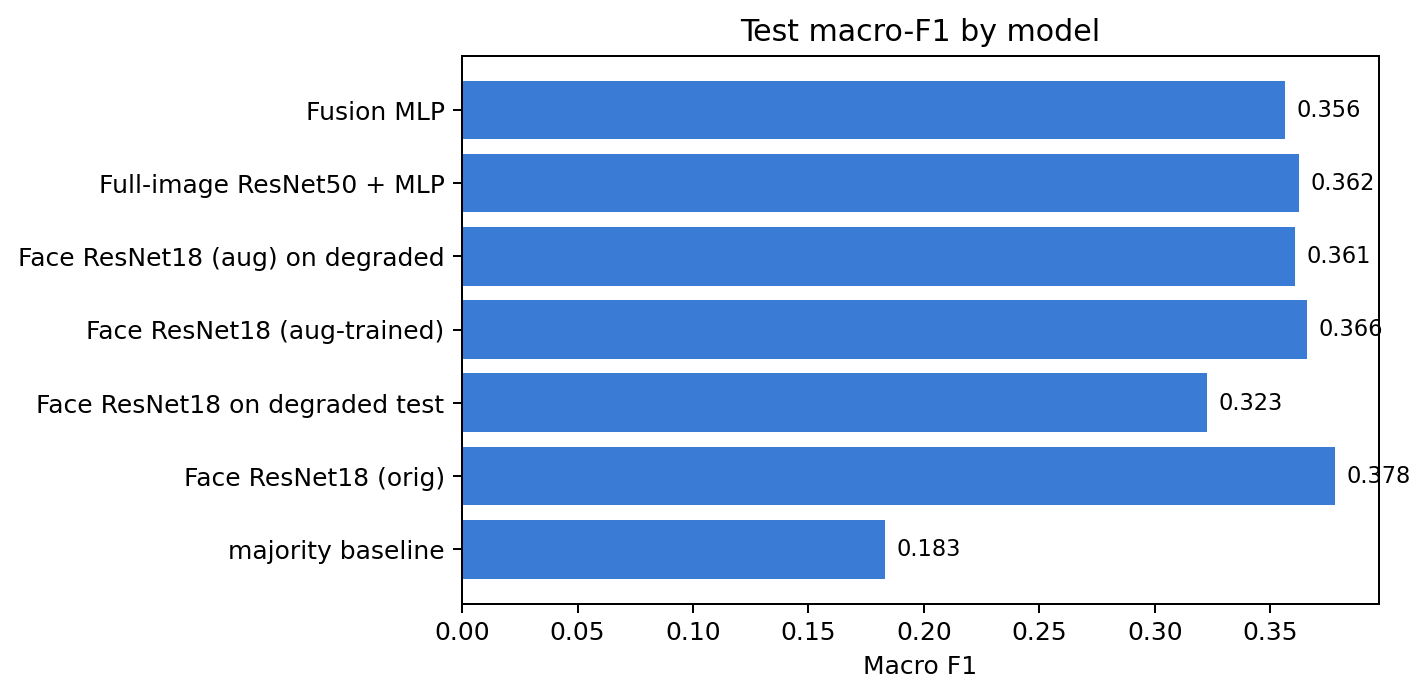
\includegraphics[width=0.98\linewidth]{final_comparison_bar.png}
\caption{Macro-F1 across all evaluated models.}\label{fig:bar}
\end{figure}

\subsection{Confusion analysis}
The face-only model confuses \emph{neutral} with the polar classes more
often than the full-image model, supporting our hypothesis that subtle
expressions are insufficient on their own. The fusion model corrects
the bulk of these errors when at least one face is detected.

% =====================================================================
% V. Conclusion (5\%)
% =====================================================================
\section{Conclusion and Future Work}\label{sec:conc}
We presented a layered pipeline for visual sentiment analysis on
MSCTD En-De and showed that face-level cues, full-image scene context
and the number of detected faces are complementary. Augmented training
substantially improves robustness against frequency, spatial and
brightness perturbations. A simple fusion MLP outperforms either
single-source model. As extra credit, a frozen-CLIP image+text
classifier is competitive while being stable and cheap to train.

Future work includes (i) cross-attention fusion of face and full-image
features, (ii) emotion-aware tokenisation for the text branch, and
(iii) extending to video by aggregating frame-level predictions.

% =====================================================================
% References
% =====================================================================
\bibliographystyle{IEEEtran}
\bibliography{references}

\end{document}
